\documentclass[10pt]{article}
\usepackage[utf8]{inputenc}
\usepackage{url}
\usepackage{hyperref}
\usepackage{amsmath}
\usepackage{amsfonts}
\usepackage{amssymb}
\usepackage{graphicx}
\graphicspath{ {./images/} }
\usepackage{float}
\usepackage{lipsum}
\usepackage{sectsty}
\sectionfont{\centering}
\usepackage{multicol}
\usepackage{xcolor}
\usepackage{natbib}
\usepackage{graphicx}
\usepackage{listings}
\usepackage{xcolor}
\usepackage{pgfplots}
\usepackage[font=small]{caption}
\addtolength{\abovecaptionskip}{-3mm}
\addtolength{\textfloatsep}{-5mm}
\setlength\columnsep{20pt}

\usepackage[a4paper,left=1.50cm, right=1.50cm, top=2cm, bottom=3cm]{geometry}


\author{}

\title{\Large{Design and Analysis of Algorithms Assignment - 6}}

\begin{document}

	\begin{center}
		{\Large \textbf{Design and Analysis of Algorithms Assignment - 6}}\\
		\vspace{1em}
		{\large Department of Information Technology,}\\
		\vspace{1em}
		\large{Indian Institute of Information Technology, Allahabad 211015, India}\\
		\vspace{1em}
		\large{SUBHASH BALLA(IIT2019207), DHANUSH VASA (IIT2019208)}
		\vspace{2.5em}

	\end{center}

%\begin{multicols*}{2}


\section*{INTRODUCTION}

We are given  an un-directed weighted graph.our goal is to find build  minimum spanning tree using kruskal's algorithm.

\textbf{Minimum Spanning Tree}- A sub graph(basically a tree)made from set of edges of input graph G(m,n) such that the graph still remains connected and sum of weights of all edges is minimum.
MST's have a lot of  practical applications in real world.


\section*{ALGORITHM DESIGN}

Given graph is, \textbf{G(m,n)}\\
\textbf{m} -set of edges with correspong weighrs\\
\textbf{n} -set of vertices\\\\
Kruskal's Algorithm is based on \textbf{cyclic property of graphs}.\\
Firstly,we sort all edges with respect to weights in \textbf{ascending order}.Then we consider each edge sequentially and check if those 2 vertices forming that edge are in same set or not.\\
If they are in same set,then including that edge creates a cycle which we don't want, since  those 2 vertices are already connected,including that edge is useless.Hence we exclude that edge.\\
If they belong to 2 different sets ,we include that edge in our MST and combine those 2 sets.\\
We use\textbf{ disjoint-set-union(DSU) data structure} to work with sets.



\lstset { %
    language=C++,
    backgroundcolor=\color{black!5},
    basicstyle=\footnotesize,
}
\section*{Code Implementation}
\lstset { %
    language=C++,
    backgroundcolor=\color{black!5},
    basicstyle=\footnotesize,
}
\begin{lstlisting}

#include<bits/stdc++.h>
using namespace std;
#define IOS ios_base::sync_with_stdio(false),cin.tie(NULL)
#define mod 1000000007
#define  pb push_back
typedef long long ll;
typedef unsigned long long ull;
typedef  long double ld;
typedef vector<int> vi;
typedef vector<bool> vb;
typedef vector<vi >vvi;
typedef vector<ll> vll;
typedef vector<vll >vvll;


struct edge_ {
	ll v1, v2, wt;
};

ll max_vertices = 25, max_weights = 10;
ll n, m, u, v, w, cost;
ll _rank[1001], par[1001];
vector<edge_>edges, result;


void create_random_graph() {

	n = 50 + rand() % max_vertices;
	ll max_edges = n * (n - 1) / 2;
	m = 1 + rand() % max_edges;


	ll edge_count = m;
	set<pair<ll, ll> >s;

	while (edge_count) {
		ll v1 = 1 + rand() % n, v2 = 1 + rand() % n;
		if (v1 == v2)continue;
		if (s.find({v1, v2}) != s.end() || s.find({v2, v1}) != s.end())continue;
		ll wt = 1 + rand() % max_weights;
		edges.pb({v1, v2, wt});
		s.insert({v1, v2});
		edge_count--;
	}

}


bool comp(const edge_ &e1, const edge_ &e2) {
	return (e1.wt < e2.wt);
}

ll find(ll v1) {

	if (par[v1] == -1)return v1;

	return par[v1] = find(par[v1]);
}

void combine(ll v1, ll v2) {

	ll a = find(v1), b = find(v2);

	if (_rank[a] == _rank[b])_rank[b]++, par[a] = b;
	if (_rank[a] < _rank[b])par[a] = b;
	else par[b] = a;
}


int main() {

	srand(time(0));

	create_random_graph();

	cout << "n  ---> " << n << "\n";
	cout << "m  ---> " << m << "\n";
	cout << "\ninput graph-->\n";
	for (auto ele : edges)cout << ele.v1 << " " << ele.v2 << " " << ele.wt << "\n";


	for (ll i = 0; i <= n; i++)par[i] = -1;

	sort(edges.begin(), edges.end(), comp);


	for (ll i = 0; i < m; i++) {
		ll v1 = edges[i].v1, v2 = edges[i].v2;
		ll a = find(v1), b = find(v2);
		if (a != b) {
			combine(a, b);
			result.pb({v1, v2, edges[i].wt});
			cost += edges[i].wt;
		}
	}

	cout << "\ncost --> " << cost << "\n";
	cout << "\nminimum spanning forest --->\n";

	for (auto ele : result)cout << ele.v1 << " " << ele.v2 << " " << ele.wt << "\n";

}

\end{lstlisting}




\section*{ALGORITHM ANALYSIS}


\rule{9cm}{1pt}\\
{
 \textbf{ Time-}\\
    \textbf{ sorting step} -\(O(m*log(m))\).\\
     For each check if both vertices belong to same set or not(find() in dsu) and combine 2 sets (union() in dsu) if they belong to different sets.\\

   In our implementation of DSU,we used both\textbf{ rank-heursitic} and \textbf{path compression technique}.\\
  Hence find() and union() works in \(\alpha(m,n)\) time,where \(\alpha(m,n)\) is inverse ackermann function.\\
  It doesn't cross '5' for any practically large real input.\\
  Hence \textbf{time taken}\textbf{=\(O(m*log(m)+m*\alpha(m,n))\)}.\\\\
 \textbf{Space- }\\
 We used rank[] and parent[] arrays to work with sets ,which are linear.\\
 Hence,\textbf{Auxillary space} =\(O(m+n)\)\\


 }
\rule{9cm}{1pt}

\section{Experimental Analysis}
In the following table some cases are plotted for the first algorithm,\newline
\begin{center}
 \begin{tabular}{||c | c | c||}
 \hline
 m & n & Time Taken (in ms) \\ [0.5ex]
 \hline\hline
 50 & 662 & 0.0000 \\
 \hline
 100 & 4011 & 0.0000 \\
 \hline
 500 & 22238 & 0.03 \\
 \hline
 1000 & 497566 & 4.89 \\
 \hline
 2000 & 900937 & 5.12 \\
 \hline
\end{tabular}
\end{center}

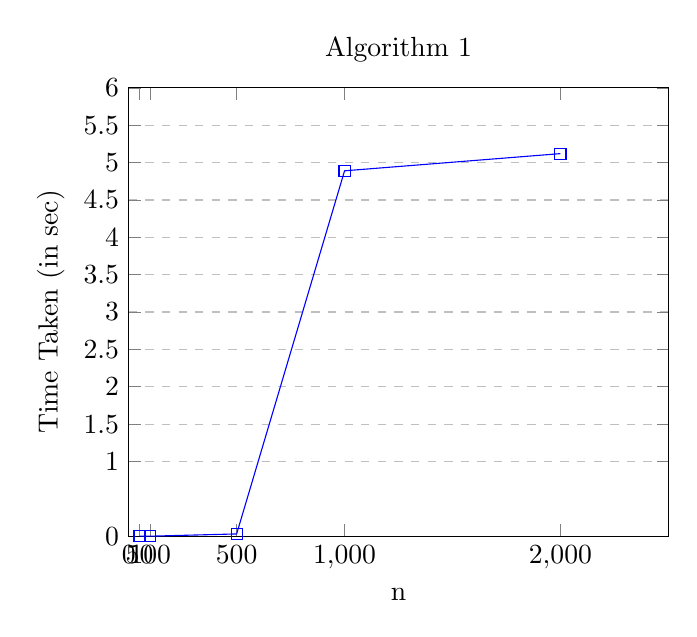
\begin{tikzpicture}
\begin{axis}[
    title={Algorithm 1},
    xlabel={n},
    ylabel={Time Taken (in sec)},
    xmin=0, xmax=2500,
    ymin=0, ymax=6.000,
    xtick={0,50,100,500,1000,2000},
    ytick={0,1,1.5,2,2.5,3,3.5,4,4.5,5,5.5,6},
    legend pos=north west,
    ymajorgrids=true,
    grid style=dashed,
]

\addplot[
    color=blue,
    mark=square,
    ]
    coordinates {
    (50,0.0000)(100,0.0000)(500,0.03)(1000,4.89)(2000,5.12)
    };


 \iffalse
 \section{Experimental Analysis}
In the following table some cases are plotted for the first algorithm,\newline
\begin{center}
 \begin{tabular}{||c | c | c||}
 \hline
 m & n & Time Taken (in ms) \\ [0.5ex]
 \hline\hline
 10 & 10 & 0.0000 \\
 \hline
 50 & 50 & 0.0000 \\
 \hline
 100 & 100 & 0.0000 \\
 \hline
 500 & 500 & 0.0500 \\
 \hline
 700 & 700 & 0.0600 \\
 \hline
 800 & 800 & 0.0700 \\
 \hline
 900 & 900 & 0.1200 \\
 \hline
 1000 & 1000 & 0.1400 \\
 \hline
 2000 & 2000 & 0.4800 \\
 \hline
 5000 & 5000 & 2.2800 \\ [1ex]
 \hline
\end{tabular}
\end{center}

\begin{tikzpicture}
\begin{axis}[
    title={Algorithm 1},
    xlabel={n},
    ylabel={Time Taken (in sec)},
    xmin=0, xmax=5000,
    ymin=0, ymax=2.3000,
    xtick={0,10,50,100,500,700,800,900,1000,2000,5000},
    ytick={0,0.0100, 0.0500, 0.1000, 0.1500, 0.2000, 0.3000,0.4000,0.5000,1.0000,2.000,2.5000},
    legend pos=north west,
    ymajorgrids=true,
    grid style=dashed,
]

\addplot[
    color=blue,
    mark=square,
    ]
    coordinates {
    (10,0.0000)(50,0.0000)(100,0.0000)(500,0.0500)(700,0.0600)(800,0.0700)(900,0.1200)(1000,0.1400)(2000,0.4800)(5000,2.2800)
    };
 \fi
\end{axis}
\end{tikzpicture}\newline


 \section*{Discussion on Parallelising Kruskal's Algorithm }\\

Kruskal's algorithm involves\\
1. sorting step.\\
2. determing if 2 vertices belong to same set or not and combine if belong to different sets.\\
Second task is difficult to parallelise .Because ,say 2 edges are being checked for that condition and calling a union() function by 2 different processors simultaneously,we could get incorrect results for find() and there is possibility that we combine 2 incorrect sets.\\
This is due to concurrency issues when working with multi processor systems.\\\\

However,\textbf{sorting step can be parallelised.}\\
Sorting can be done in \textbf{linear time} if worked with \textbf{O(log(m)) processors}.\\\\

Hence \textbf{Time taken} = O(n+m*\alpha(m,n)) = O(m*\alpha(m,n)).\\\\

 This is better than usual serial kruskal's algorithm.\\

\iffalse
\section*{APPLICATIONS}
Divide and Conquer is a wide variety of algorithmic technique which solves difficult problems with ease.these are efficient when compared with counterpart brute-force approach.it do not needs any modifications .this strategy uses recursion that makes it a little slower. Some of the applications of the Divide and Conquer Approach are:

\begin{enumerate}
\item \textbf{Merge Sort}
\item \textbf{Quick Sort}
\item \textbf{Binary Search}
\item \textbf{Segment Trees}
\item  \textbf{Strassen’s Algorithm} etc many more.\fi
\end{enumerate}

\section*{CONCLUSION}

We can conclude that the given problem of finding minimum spanning tree(MST) of a given graph works in \(O(m*log(m)+m*\alpha(m,n))\)} time and consumes \(O(m+n)\) space.\\

\section*{ACKNOWLEDGMENT}

We are very much grateful to our Course instructor Mr.Rahul Kala and our mentor, Ms.Tejasvee, who have provided the great opportunity to do this wonderful work on the subject of Design and Analysis of Algorithms, specifically on MST's and kruskal's algorithm.


\section*{REFERENCES}
1.https://en.wikipedia.org/wiki/Kruskal\%27s_algorithm

\end{enumerate}

%\end{multicols*}

\end{document}
